\documentclass[1p]{elsarticle_modified}
%\bibliographystyle{elsarticle-num}

%\usepackage[colorlinks]{hyperref}
%\usepackage{abbrmath_seonhwa} %\Abb, \Ascr, \Acal ,\Abf, \Afrak
\usepackage{amsfonts}
\usepackage{amssymb}
\usepackage{amsmath}
\usepackage{amsthm}
\usepackage{scalefnt}
\usepackage{amsbsy}
\usepackage{kotex}
\usepackage{caption}
\usepackage{subfig}
\usepackage{color}
\usepackage{graphicx}
\usepackage{xcolor} %% white, black, red, green, blue, cyan, magenta, yellow
\usepackage{float}
\usepackage{setspace}
\usepackage{hyperref}

\usepackage{tikz}
\usetikzlibrary{arrows}

\usepackage{multirow}
\usepackage{array} % fixed length table
\usepackage{hhline}

%%%%%%%%%%%%%%%%%%%%%
\makeatletter
\renewcommand*\env@matrix[1][\arraystretch]{%
	\edef\arraystretch{#1}%
	\hskip -\arraycolsep
	\let\@ifnextchar\new@ifnextchar
	\array{*\c@MaxMatrixCols c}}
\makeatother %https://tex.stackexchange.com/questions/14071/how-can-i-increase-the-line-spacing-in-a-matrix
%%%%%%%%%%%%%%%

\usepackage[normalem]{ulem}

\newcommand{\msout}[1]{\ifmmode\text{\sout{\ensuremath{#1}}}\else\sout{#1}\fi}
%SOURCE: \msout is \stkout macro in https://tex.stackexchange.com/questions/20609/strikeout-in-math-mode

\newcommand{\cancel}[1]{
	\ifmmode
	{\color{red}\msout{#1}}
	\else
	{\color{red}\sout{#1}}
	\fi
}

\newcommand{\add}[1]{
	{\color{blue}\uwave{#1}}
}

\newcommand{\replace}[2]{
	\ifmmode
	{\color{red}\msout{#1}}{\color{blue}\uwave{#2}}
	\else
	{\color{red}\sout{#1}}{\color{blue}\uwave{#2}}
	\fi
}

\newcommand{\Sol}{\mathcal{S}} %segment
\newcommand{\D}{D} %diagram
\newcommand{\A}{\mathcal{A}} %arc


%%%%%%%%%%%%%%%%%%%%%%%%%%%%%5 test

\def\sl{\operatorname{\textup{SL}}(2,\Cbb)}
\def\psl{\operatorname{\textup{PSL}}(2,\Cbb)}
\def\quan{\mkern 1mu \triangleright \mkern 1mu}

\theoremstyle{definition}
\newtheorem{thm}{Theorem}[section]
\newtheorem{prop}[thm]{Proposition}
\newtheorem{lem}[thm]{Lemma}
\newtheorem{ques}[thm]{Question}
\newtheorem{cor}[thm]{Corollary}
\newtheorem{defn}[thm]{Definition}
\newtheorem{exam}[thm]{Example}
\newtheorem{rmk}[thm]{Remark}
\newtheorem{alg}[thm]{Algorithm}

\newcommand{\I}{\sqrt{-1}}
\begin{document}

%\begin{frontmatter}
%
%\title{Boundary parabolic representations of knots up to 8 crossings}
%
%%% Group authors per affiliation:
%\author{Yunhi Cho} 
%\address{Department of Mathematics, University of Seoul, Seoul, Korea}
%\ead{yhcho@uos.ac.kr}
%
%
%\author{Seonhwa Kim} %\fnref{s_kim}}
%\address{Center for Geometry and Physics, Institute for Basic Science, Pohang, 37673, Korea}
%\ead{ryeona17@ibs.re.kr}
%
%\author{Hyuk Kim}
%\address{Department of Mathematical Sciences, Seoul National University, Seoul 08826, Korea}
%\ead{hyukkim@snu.ac.kr}
%
%\author{Seokbeom Yoon}
%\address{Department of Mathematical Sciences, Seoul National University, Seoul, 08826,  Korea}
%\ead{sbyoon15@snu.ac.kr}
%
%\begin{abstract}
%We find all boundary parabolic representation of knots up to 8 crossings.
%
%\end{abstract}
%\begin{keyword}
%    \MSC[2010] 57M25 
%\end{keyword}
%
%\end{frontmatter}

%\linenumbers
%\tableofcontents
%
\newcommand\colored[1]{\textcolor{white}{\rule[-0.35ex]{0.8em}{1.4ex}}\kern-0.8em\color{red} #1}%
%\newcommand\colored[1]{\textcolor{white}{ #1}\kern-2.17ex	\textcolor{white}{ #1}\kern-1.81ex	\textcolor{white}{ #1}\kern-2.15ex\color{red}#1	}

{\Large $\underline{11n_{48}~(K11n_{48})}$}

\setlength{\tabcolsep}{10pt}
\renewcommand{\arraystretch}{1.6}
\vspace{1cm}\begin{tabular}{m{100pt}>{\centering\arraybackslash}m{274pt}}
\multirow{5}{120pt}{
	\centering
	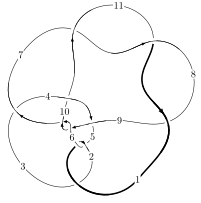
\includegraphics[width=112pt]{../../../GIT/diagram.site/Diagrams/png/664_11n_48.png}\\
\ \ \ A knot diagram\footnotemark}&
\allowdisplaybreaks
\textbf{Linearized knot diagam} \\
\cline{2-2}
 &
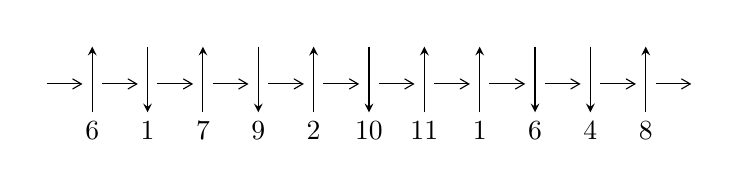
\begin{tikzpicture}[x=20pt, y=17pt]
	% nodes
	\node (C0) at (0, 0) {};
	\node (C1) at (1, 0) {};
	\node (C1U) at (1, +1) {};
	\node (C1D) at (1, -1) {6};

	\node (C2) at (2, 0) {};
	\node (C2U) at (2, +1) {};
	\node (C2D) at (2, -1) {1};

	\node (C3) at (3, 0) {};
	\node (C3U) at (3, +1) {};
	\node (C3D) at (3, -1) {7};

	\node (C4) at (4, 0) {};
	\node (C4U) at (4, +1) {};
	\node (C4D) at (4, -1) {9};

	\node (C5) at (5, 0) {};
	\node (C5U) at (5, +1) {};
	\node (C5D) at (5, -1) {2};

	\node (C6) at (6, 0) {};
	\node (C6U) at (6, +1) {};
	\node (C6D) at (6, -1) {10};

	\node (C7) at (7, 0) {};
	\node (C7U) at (7, +1) {};
	\node (C7D) at (7, -1) {11};

	\node (C8) at (8, 0) {};
	\node (C8U) at (8, +1) {};
	\node (C8D) at (8, -1) {1};

	\node (C9) at (9, 0) {};
	\node (C9U) at (9, +1) {};
	\node (C9D) at (9, -1) {6};

	\node (C10) at (10, 0) {};
	\node (C10U) at (10, +1) {};
	\node (C10D) at (10, -1) {4};

	\node (C11) at (11, 0) {};
	\node (C11U) at (11, +1) {};
	\node (C11D) at (11, -1) {8};
	\node (C12) at (12, 0) {};

	% arrows
	\draw[->,>={angle 60}]
	(C0) edge (C1) (C1) edge (C2) (C2) edge (C3) (C3) edge (C4) (C4) edge (C5) (C5) edge (C6) (C6) edge (C7) (C7) edge (C8) (C8) edge (C9) (C9) edge (C10) (C10) edge (C11) (C11) edge (C12) ;	\draw[->,>=stealth]
	(C1D) edge (C1U) (C2U) edge (C2D) (C3D) edge (C3U) (C4U) edge (C4D) (C5D) edge (C5U) (C6U) edge (C6D) (C7D) edge (C7U) (C8D) edge (C8U) (C9U) edge (C9D) (C10U) edge (C10D) (C11D) edge (C11U) ;
	\end{tikzpicture} \\
\hhline{~~} \\& 
\textbf{Solving Sequence} \\ \cline{2-2} 
 &
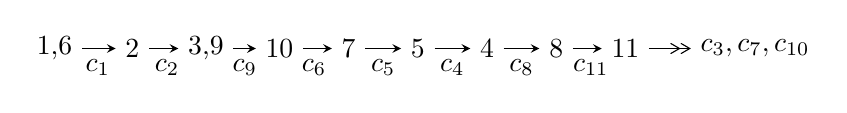
\begin{tikzpicture}[x=25pt, y=7pt]
	% node
	\node (A0) at (-1/8, 0) {1,6};
	\node (A1) at (1, 0) {2};
	\node (A2) at (33/16, 0) {3,9};
	\node (A3) at (25/8, 0) {10};
	\node (A4) at (33/8, 0) {7};
	\node (A5) at (41/8, 0) {5};
	\node (A6) at (49/8, 0) {4};
	\node (A7) at (57/8, 0) {8};
	\node (A8) at (65/8, 0) {11};
	\node (C1) at (1/2, -1) {$c_{1}$};
	\node (C2) at (3/2, -1) {$c_{2}$};
	\node (C3) at (21/8, -1) {$c_{9}$};
	\node (C4) at (29/8, -1) {$c_{6}$};
	\node (C5) at (37/8, -1) {$c_{5}$};
	\node (C6) at (45/8, -1) {$c_{4}$};
	\node (C7) at (53/8, -1) {$c_{8}$};
	\node (C8) at (61/8, -1) {$c_{11}$};
	\node (A9) at (10, 0) {$c_{3},c_{7},c_{10}$};

	% edge
	\draw[->,>=stealth]	
	(A0) edge (A1) (A1) edge (A2) (A2) edge (A3) (A3) edge (A4) (A4) edge (A5) (A5) edge (A6) (A6) edge (A7) (A7) edge (A8) ;
	\draw[->>,>={angle 60}]	
	(A8) edge (A9);
\end{tikzpicture} \\ 

\end{tabular} \\

\footnotetext{
The image of knot diagram is generated by the software ``\textbf{Draw programme}" developed by Andrew Bartholomew(\url{http://www.layer8.co.uk/maths/draw/index.htm\#Running-draw}), where we modified some parts for our purpose(\url{https://github.com/CATsTAILs/LinksPainter}).
}\phantom \\ \newline 
\centering \textbf{Ideals for irreducible components\footnotemark of $X_{\text{par}}$} 
 
\begin{align*}
I^u_{1}&=\langle 
-1.14153\times10^{15} u^{19}-4.26909\times10^{15} u^{18}+\cdots+8.56391\times10^{15} b+1.10053\times10^{16},\\
\phantom{I^u_{1}}&\phantom{= \langle  }6.37825\times10^{15} u^{19}+2.69128\times10^{16} u^{18}+\cdots+8.56391\times10^{15} a+3.19918\times10^{16},\;u^{20}+4 u^{19}+\cdots+2 u+1\rangle \\
I^u_{2}&=\langle 
b^2-2,\;a+u+1,\;u^2+u+1\rangle \\
I^u_{3}&=\langle 
b,\;a- u-1,\;u^2+u+1\rangle \\
\\
\end{align*}
\raggedright * 3 irreducible components of $\dim_{\mathbb{C}}=0$, with total 26 representations.\\
\footnotetext{All coefficients of polynomials are rational numbers. But the coefficients are sometimes approximated in decimal forms when there is not enough margin.}
\newpage
\renewcommand{\arraystretch}{1}
\centering \section*{I. $I^u_{1}= \langle -1.14\times10^{15} u^{19}-4.27\times10^{15} u^{18}+\cdots+8.56\times10^{15} b+1.10\times10^{16},\;6.38\times10^{15} u^{19}+2.69\times10^{16} u^{18}+\cdots+8.56\times10^{15} a+3.20\times10^{16},\;u^{20}+4 u^{19}+\cdots+2 u+1 \rangle$}
\flushleft \textbf{(i) Arc colorings}\\
\begin{tabular}{m{7pt} m{180pt} m{7pt} m{180pt} }
\flushright $a_{1}=$&$\begin{pmatrix}1\\0\end{pmatrix}$ \\
\flushright $a_{6}=$&$\begin{pmatrix}0\\u\end{pmatrix}$ \\
\flushright $a_{2}=$&$\begin{pmatrix}1\\- u^2\end{pmatrix}$ \\
\flushright $a_{3}=$&$\begin{pmatrix}u^2+1\\- u^2\end{pmatrix}$ \\
\flushright $a_{9}=$&$\begin{pmatrix}-0.744782 u^{19}-3.14258 u^{18}+\cdots-36.0811 u-3.73565\\0.133295 u^{19}+0.498498 u^{18}+\cdots+1.29523 u-1.28508\end{pmatrix}$ \\
\flushright $a_{10}=$&$\begin{pmatrix}-0.744782 u^{19}-3.14258 u^{18}+\cdots-36.0811 u-3.73565\\0.169440 u^{19}+0.644676 u^{18}+\cdots+2.36692 u-1.12163\end{pmatrix}$ \\
\flushright $a_{7}=$&$\begin{pmatrix}0.408694 u^{19}+1.81167 u^{18}+\cdots+31.0989 u+4.13465\\-0.233980 u^{19}-0.931452 u^{18}+\cdots-3.19070 u+0.665806\end{pmatrix}$ \\
\flushright $a_{5}=$&$\begin{pmatrix}- u\\u^3+u\end{pmatrix}$ \\
\flushright $a_{4}=$&$\begin{pmatrix}-0.174714 u^{19}-0.880217 u^{18}+\cdots-27.9082 u-4.80045\\0.258642 u^{19}+1.02897 u^{18}+\cdots+6.32631 u-0.537037\end{pmatrix}$ \\
\flushright $a_{8}=$&$\begin{pmatrix}-0.878077 u^{19}-3.64108 u^{18}+\cdots-37.3764 u-2.45056\\0.133295 u^{19}+0.498498 u^{18}+\cdots+1.29523 u-1.28508\end{pmatrix}$ \\
\flushright $a_{11}=$&$\begin{pmatrix}1.12163 u^{19}+4.65596 u^{18}+\cdots+50.9286 u+4.61018\\-0.278931 u^{19}-1.06850 u^{18}+\cdots-2.73563 u+1.50344\end{pmatrix}$\\ \flushright $a_{11}=$&$\begin{pmatrix}1.12163 u^{19}+4.65596 u^{18}+\cdots+50.9286 u+4.61018\\-0.278931 u^{19}-1.06850 u^{18}+\cdots-2.73563 u+1.50344\end{pmatrix}$\\&\end{tabular}
\flushleft \textbf{(ii) Obstruction class $= -1$}\\~\\
\flushleft \textbf{(iii) Cusp Shapes $= -\frac{1557563512851975}{8563912733265916} u^{19}-\frac{8797950809282545}{8563912733265916} u^{18}+\cdots-\frac{62067062106158523}{8563912733265916} u-\frac{1550791485072395}{2140978183316479}$}\\~\\
\newpage\renewcommand{\arraystretch}{1}
\flushleft \textbf{(iv) u-Polynomials at the component}\newline \\
\begin{tabular}{m{50pt}|m{274pt}}
Crossings & \hspace{64pt}u-Polynomials at each crossing \\
\hline $$\begin{aligned}c_{1},c_{5}\end{aligned}$$&$\begin{aligned}
&u^{20}-4 u^{19}+\cdots-2 u+1
\end{aligned}$\\
\hline $$\begin{aligned}c_{2}\end{aligned}$$&$\begin{aligned}
&u^{20}+28 u^{19}+\cdots+74 u+1
\end{aligned}$\\
\hline $$\begin{aligned}c_{3}\end{aligned}$$&$\begin{aligned}
&u^{20}+8 u^{18}+\cdots-16 u+41
\end{aligned}$\\
\hline $$\begin{aligned}c_{4}\end{aligned}$$&$\begin{aligned}
&u^{20}-2 u^{19}+\cdots+2204 u+839
\end{aligned}$\\
\hline $$\begin{aligned}c_{6},c_{9}\end{aligned}$$&$\begin{aligned}
&u^{20}+3 u^{19}+\cdots-19 u+7
\end{aligned}$\\
\hline $$\begin{aligned}c_{7},c_{8},c_{11}\end{aligned}$$&$\begin{aligned}
&u^{20}- u^{19}+\cdots-12 u+4
\end{aligned}$\\
\hline $$\begin{aligned}c_{10}\end{aligned}$$&$\begin{aligned}
&u^{20}+2 u^{19}+\cdots-2 u+1
\end{aligned}$\\
\hline
\end{tabular}\\~\\
\newpage\renewcommand{\arraystretch}{1}
\flushleft \textbf{(v) Riley Polynomials at the component}\newline \\
\begin{tabular}{m{50pt}|m{274pt}}
Crossings & \hspace{64pt}Riley Polynomials at each crossing \\
\hline $$\begin{aligned}c_{1},c_{5}\end{aligned}$$&$\begin{aligned}
&y^{20}+28 y^{19}+\cdots+74 y+1
\end{aligned}$\\
\hline $$\begin{aligned}c_{2}\end{aligned}$$&$\begin{aligned}
&y^{20}-68 y^{19}+\cdots-1654 y+1
\end{aligned}$\\
\hline $$\begin{aligned}c_{3}\end{aligned}$$&$\begin{aligned}
&y^{20}+16 y^{19}+\cdots+10814 y+1681
\end{aligned}$\\
\hline $$\begin{aligned}c_{4}\end{aligned}$$&$\begin{aligned}
&y^{20}-52 y^{19}+\cdots+5336234 y+703921
\end{aligned}$\\
\hline $$\begin{aligned}c_{6},c_{9}\end{aligned}$$&$\begin{aligned}
&y^{20}-29 y^{19}+\cdots+297 y+49
\end{aligned}$\\
\hline $$\begin{aligned}c_{7},c_{8},c_{11}\end{aligned}$$&$\begin{aligned}
&y^{20}-15 y^{19}+\cdots-48 y+16
\end{aligned}$\\
\hline $$\begin{aligned}c_{10}\end{aligned}$$&$\begin{aligned}
&y^{20}+4 y^{19}+\cdots+2 y+1
\end{aligned}$\\
\hline
\end{tabular}\\~\\
\newpage\flushleft \textbf{(vi) Complex Volumes and Cusp Shapes}
$$\begin{array}{c|c|c}  
\text{Solutions to }I^u_{1}& \I (\text{vol} + \sqrt{-1}CS) & \text{Cusp shape}\\
 \hline 
\begin{aligned}
u &= -0.729618 + 0.601963 I \\
a &= -0.002660 - 0.502436 I \\
b &= \phantom{-}1.343650 - 0.072587 I\end{aligned}
 & \phantom{-}5.16928 - 2.57908 I & \phantom{-}8.86572 + 4.96809 I \\ \hline\begin{aligned}
u &= -0.729618 - 0.601963 I \\
a &= -0.002660 + 0.502436 I \\
b &= \phantom{-}1.343650 + 0.072587 I\end{aligned}
 & \phantom{-}5.16928 + 2.57908 I & \phantom{-}8.86572 - 4.96809 I \\ \hline\begin{aligned}
u &= \phantom{-}0.337333 + 0.681420 I \\
a &= -1.15996 + 1.26131 I \\
b &= \phantom{-}0.515876 + 0.585061 I\end{aligned}
 & -3.04083 - 0.89466 I & -2.94359 - 0.44261 I \\ \hline\begin{aligned}
u &= \phantom{-}0.337333 - 0.681420 I \\
a &= -1.15996 - 1.26131 I \\
b &= \phantom{-}0.515876 - 0.585061 I\end{aligned}
 & -3.04083 + 0.89466 I & -2.94359 + 0.44261 I \\ \hline\begin{aligned}
u &= -0.342865 + 1.301010 I \\
a &= -0.567886 - 0.523820 I \\
b &= -0.778134 - 0.346045 I\end{aligned}
 & -1.166150 - 0.686038 I & \phantom{-}1.05440 - 1.40687 I \\ \hline\begin{aligned}
u &= -0.342865 - 1.301010 I \\
a &= -0.567886 + 0.523820 I \\
b &= -0.778134 + 0.346045 I\end{aligned}
 & -1.166150 + 0.686038 I & \phantom{-}1.05440 + 1.40687 I \\ \hline\begin{aligned}
u &= -0.007874 + 1.394550 I \\
a &= \phantom{-}0.585444 - 0.602506 I \\
b &= \phantom{-}1.027390 - 0.480106 I\end{aligned}
 & -1.53618 - 5.13397 I & \phantom{-}0.62229 + 5.85487 I \\ \hline\begin{aligned}
u &= -0.007874 - 1.394550 I \\
a &= \phantom{-}0.585444 + 0.602506 I \\
b &= \phantom{-}1.027390 + 0.480106 I\end{aligned}
 & -1.53618 + 5.13397 I & \phantom{-}0.62229 - 5.85487 I \\ \hline\begin{aligned}
u &= -1.10251 + 0.94498 I \\
a &= \phantom{-}0.757275 + 0.607433 I \\
b &= -0.965691 + 0.331710 I\end{aligned}
 & -0.59440 - 3.60439 I & \phantom{-}2.12405 + 4.48047 I \\ \hline\begin{aligned}
u &= -1.10251 - 0.94498 I \\
a &= \phantom{-}0.757275 - 0.607433 I \\
b &= -0.965691 - 0.331710 I\end{aligned}
 & -0.59440 + 3.60439 I & \phantom{-}2.12405 - 4.48047 I\\
 \hline 
 \end{array}$$\newpage$$\begin{array}{c|c|c}  
\text{Solutions to }I^u_{1}& \I (\text{vol} + \sqrt{-1}CS) & \text{Cusp shape}\\
 \hline 
\begin{aligned}
u &= -0.195248 + 0.372946 I \\
a &= -0.774007 + 0.603593 I \\
b &= -0.277579 + 0.390975 I\end{aligned}
 & \phantom{-}0.131319 - 1.058260 I & \phantom{-}2.00315 + 6.24655 I \\ \hline\begin{aligned}
u &= -0.195248 - 0.372946 I \\
a &= -0.774007 - 0.603593 I \\
b &= -0.277579 - 0.390975 I\end{aligned}
 & \phantom{-}0.131319 + 1.058260 I & \phantom{-}2.00315 - 6.24655 I \\ \hline\begin{aligned}
u &= \phantom{-}0.36556 + 1.75156 I \\
a &= -0.101116 + 1.030470 I \\
b &= \phantom{-}1.39118 + 0.66555 I\end{aligned}
 & -11.13930 + 2.93869 I & -0.922503 - 0.819894 I \\ \hline\begin{aligned}
u &= \phantom{-}0.36556 - 1.75156 I \\
a &= -0.101116 - 1.030470 I \\
b &= \phantom{-}1.39118 - 0.66555 I\end{aligned}
 & -11.13930 - 2.93869 I & -0.922503 + 0.819894 I \\ \hline\begin{aligned}
u &= \phantom{-}0.030822 + 0.170366 I \\
a &= -0.29189 - 5.45429 I \\
b &= -1.370380 + 0.067940 I\end{aligned}
 & \phantom{-}3.14870 - 0.11294 I & \phantom{-}1.81708 - 1.16761 I \\ \hline\begin{aligned}
u &= \phantom{-}0.030822 - 0.170366 I \\
a &= -0.29189 + 5.45429 I \\
b &= -1.370380 - 0.067940 I\end{aligned}
 & \phantom{-}3.14870 + 0.11294 I & \phantom{-}1.81708 + 1.16761 I \\ \hline\begin{aligned}
u &= -0.36649 + 1.92873 I \\
a &= \phantom{-}0.003517 + 0.916631 I \\
b &= -1.46300 + 0.57660 I\end{aligned}
 & -10.3499 - 9.9960 I & \phantom{-}0.04826 + 5.02986 I \\ \hline\begin{aligned}
u &= -0.36649 - 1.92873 I \\
a &= \phantom{-}0.003517 - 0.916631 I \\
b &= -1.46300 - 0.57660 I\end{aligned}
 & -10.3499 + 9.9960 I & \phantom{-}0.04826 - 5.02986 I \\ \hline\begin{aligned}
u &= \phantom{-}0.01089 + 1.99331 I \\
a &= \phantom{-}0.051284 - 0.957095 I \\
b &= \phantom{-}0.076693 - 1.208720 I\end{aligned}
 & -15.1661 - 3.6593 I & -2.66886 + 2.23636 I \\ \hline\begin{aligned}
u &= \phantom{-}0.01089 - 1.99331 I \\
a &= \phantom{-}0.051284 + 0.957095 I \\
b &= \phantom{-}0.076693 + 1.208720 I\end{aligned}
 & -15.1661 + 3.6593 I & -2.66886 - 2.23636 I\\
 \hline 
 \end{array}$$\newpage\newpage\renewcommand{\arraystretch}{1}
\centering \section*{II. $I^u_{2}= \langle b^2-2,\;a+u+1,\;u^2+u+1 \rangle$}
\flushleft \textbf{(i) Arc colorings}\\
\begin{tabular}{m{7pt} m{180pt} m{7pt} m{180pt} }
\flushright $a_{1}=$&$\begin{pmatrix}1\\0\end{pmatrix}$ \\
\flushright $a_{6}=$&$\begin{pmatrix}0\\u\end{pmatrix}$ \\
\flushright $a_{2}=$&$\begin{pmatrix}1\\u+1\end{pmatrix}$ \\
\flushright $a_{3}=$&$\begin{pmatrix}- u\\u+1\end{pmatrix}$ \\
\flushright $a_{9}=$&$\begin{pmatrix}- u-1\\b\end{pmatrix}$ \\
\flushright $a_{10}=$&$\begin{pmatrix}- u-1\\b+u\end{pmatrix}$ \\
\flushright $a_{7}=$&$\begin{pmatrix}u+1\\- b\end{pmatrix}$ \\
\flushright $a_{5}=$&$\begin{pmatrix}- u\\u+1\end{pmatrix}$ \\
\flushright $a_{4}=$&$\begin{pmatrix}b- u-1\\- b u+3 u+1\end{pmatrix}$ \\
\flushright $a_{8}=$&$\begin{pmatrix}- b- u-1\\b\end{pmatrix}$ \\
\flushright $a_{11}=$&$\begin{pmatrix}- b u- b-1\\2\end{pmatrix}$\\ \flushright $a_{11}=$&$\begin{pmatrix}- b u- b-1\\2\end{pmatrix}$\\&\end{tabular}
\flushleft \textbf{(ii) Obstruction class $= 1$}\\~\\
\flushleft \textbf{(iii) Cusp Shapes $= 4 u+4$}\\~\\
\newpage\renewcommand{\arraystretch}{1}
\flushleft \textbf{(iv) u-Polynomials at the component}\newline \\
\begin{tabular}{m{50pt}|m{274pt}}
Crossings & \hspace{64pt}u-Polynomials at each crossing \\
\hline $$\begin{aligned}c_{1},c_{2},c_{10}\end{aligned}$$&$\begin{aligned}
&(u^2+u+1)^2
\end{aligned}$\\
\hline $$\begin{aligned}c_{3}\end{aligned}$$&$\begin{aligned}
&u^4-2 u^3+5 u^2+2 u+1
\end{aligned}$\\
\hline $$\begin{aligned}c_{4}\end{aligned}$$&$\begin{aligned}
&u^4+2 u^3+5 u^2-2 u+1
\end{aligned}$\\
\hline $$\begin{aligned}c_{5}\end{aligned}$$&$\begin{aligned}
&(u^2- u+1)^2
\end{aligned}$\\
\hline $$\begin{aligned}c_{6}\end{aligned}$$&$\begin{aligned}
&(u+1)^4
\end{aligned}$\\
\hline $$\begin{aligned}c_{7},c_{8},c_{11}\end{aligned}$$&$\begin{aligned}
&(u^2-2)^2
\end{aligned}$\\
\hline $$\begin{aligned}c_{9}\end{aligned}$$&$\begin{aligned}
&(u-1)^4
\end{aligned}$\\
\hline
\end{tabular}\\~\\
\newpage\renewcommand{\arraystretch}{1}
\flushleft \textbf{(v) Riley Polynomials at the component}\newline \\
\begin{tabular}{m{50pt}|m{274pt}}
Crossings & \hspace{64pt}Riley Polynomials at each crossing \\
\hline $$\begin{aligned}c_{1},c_{2},c_{5}\\c_{10}\end{aligned}$$&$\begin{aligned}
&(y^2+y+1)^2
\end{aligned}$\\
\hline $$\begin{aligned}c_{3},c_{4}\end{aligned}$$&$\begin{aligned}
&y^4+6 y^3+35 y^2+6 y+1
\end{aligned}$\\
\hline $$\begin{aligned}c_{6},c_{9}\end{aligned}$$&$\begin{aligned}
&(y-1)^4
\end{aligned}$\\
\hline $$\begin{aligned}c_{7},c_{8},c_{11}\end{aligned}$$&$\begin{aligned}
&(y-2)^4
\end{aligned}$\\
\hline
\end{tabular}\\~\\
\newpage\flushleft \textbf{(vi) Complex Volumes and Cusp Shapes}
$$\begin{array}{c|c|c}  
\text{Solutions to }I^u_{2}& \I (\text{vol} + \sqrt{-1}CS) & \text{Cusp shape}\\
 \hline 
\begin{aligned}
u &= -0.500000 + 0.866025 I \\
a &= -0.500000 - 0.866025 I \\
b &= \phantom{-}1.41421\phantom{ +0.000000I}\end{aligned}
 & \phantom{-}3.28987 - 2.02988 I & \phantom{-}2.00000 + 3.46410 I \\ \hline\begin{aligned}
u &= -0.500000 + 0.866025 I \\
a &= -0.500000 - 0.866025 I \\
b &= -1.41421\phantom{ +0.000000I}\end{aligned}
 & \phantom{-}3.28987 - 2.02988 I & \phantom{-}2.00000 + 3.46410 I \\ \hline\begin{aligned}
u &= -0.500000 - 0.866025 I \\
a &= -0.500000 + 0.866025 I \\
b &= \phantom{-}1.41421\phantom{ +0.000000I}\end{aligned}
 & \phantom{-}3.28987 + 2.02988 I & \phantom{-}2.00000 - 3.46410 I \\ \hline\begin{aligned}
u &= -0.500000 - 0.866025 I \\
a &= -0.500000 + 0.866025 I \\
b &= -1.41421\phantom{ +0.000000I}\end{aligned}
 & \phantom{-}3.28987 + 2.02988 I & \phantom{-}2.00000 - 3.46410 I\\
 \hline 
 \end{array}$$\newpage\newpage\renewcommand{\arraystretch}{1}
\centering \section*{III. $I^u_{3}= \langle b,\;a- u-1,\;u^2+u+1 \rangle$}
\flushleft \textbf{(i) Arc colorings}\\
\begin{tabular}{m{7pt} m{180pt} m{7pt} m{180pt} }
\flushright $a_{1}=$&$\begin{pmatrix}1\\0\end{pmatrix}$ \\
\flushright $a_{6}=$&$\begin{pmatrix}0\\u\end{pmatrix}$ \\
\flushright $a_{2}=$&$\begin{pmatrix}1\\u+1\end{pmatrix}$ \\
\flushright $a_{3}=$&$\begin{pmatrix}- u\\u+1\end{pmatrix}$ \\
\flushright $a_{9}=$&$\begin{pmatrix}u+1\\0\end{pmatrix}$ \\
\flushright $a_{10}=$&$\begin{pmatrix}u+1\\- u\end{pmatrix}$ \\
\flushright $a_{7}=$&$\begin{pmatrix}u+1\\0\end{pmatrix}$ \\
\flushright $a_{5}=$&$\begin{pmatrix}- u\\u+1\end{pmatrix}$ \\
\flushright $a_{4}=$&$\begin{pmatrix}- u-1\\u+1\end{pmatrix}$ \\
\flushright $a_{8}=$&$\begin{pmatrix}u+1\\0\end{pmatrix}$ \\
\flushright $a_{11}=$&$\begin{pmatrix}1\\0\end{pmatrix}$\\ \flushright $a_{11}=$&$\begin{pmatrix}1\\0\end{pmatrix}$\\&\end{tabular}
\flushleft \textbf{(ii) Obstruction class $= 1$}\\~\\
\flushleft \textbf{(iii) Cusp Shapes $= 4 u+2$}\\~\\
\newpage\renewcommand{\arraystretch}{1}
\flushleft \textbf{(iv) u-Polynomials at the component}\newline \\
\begin{tabular}{m{50pt}|m{274pt}}
Crossings & \hspace{64pt}u-Polynomials at each crossing \\
\hline $$\begin{aligned}c_{1},c_{2}\end{aligned}$$&$\begin{aligned}
&u^2+u+1
\end{aligned}$\\
\hline $$\begin{aligned}c_{3},c_{4},c_{5}\\c_{10}\end{aligned}$$&$\begin{aligned}
&u^2- u+1
\end{aligned}$\\
\hline $$\begin{aligned}c_{6}\end{aligned}$$&$\begin{aligned}
&(u-1)^2
\end{aligned}$\\
\hline $$\begin{aligned}c_{7},c_{8},c_{11}\end{aligned}$$&$\begin{aligned}
&u^2
\end{aligned}$\\
\hline $$\begin{aligned}c_{9}\end{aligned}$$&$\begin{aligned}
&(u+1)^2
\end{aligned}$\\
\hline
\end{tabular}\\~\\
\newpage\renewcommand{\arraystretch}{1}
\flushleft \textbf{(v) Riley Polynomials at the component}\newline \\
\begin{tabular}{m{50pt}|m{274pt}}
Crossings & \hspace{64pt}Riley Polynomials at each crossing \\
\hline $$\begin{aligned}c_{1},c_{2},c_{3}\\c_{4},c_{5},c_{10}\end{aligned}$$&$\begin{aligned}
&y^2+y+1
\end{aligned}$\\
\hline $$\begin{aligned}c_{6},c_{9}\end{aligned}$$&$\begin{aligned}
&(y-1)^2
\end{aligned}$\\
\hline $$\begin{aligned}c_{7},c_{8},c_{11}\end{aligned}$$&$\begin{aligned}
&y^2
\end{aligned}$\\
\hline
\end{tabular}\\~\\
\newpage\flushleft \textbf{(vi) Complex Volumes and Cusp Shapes}
$$\begin{array}{c|c|c}  
\text{Solutions to }I^u_{3}& \I (\text{vol} + \sqrt{-1}CS) & \text{Cusp shape}\\
 \hline 
\begin{aligned}
u &= -0.500000 + 0.866025 I \\
a &= \phantom{-}0.500000 + 0.866025 I \\
b &= \phantom{-0.000000 } 0\end{aligned}
 & -1.64493 - 2.02988 I & \phantom{-0.000000 -}0. + 3.46410 I \\ \hline\begin{aligned}
u &= -0.500000 - 0.866025 I \\
a &= \phantom{-}0.500000 - 0.866025 I \\
b &= \phantom{-0.000000 } 0\end{aligned}
 & -1.64493 + 2.02988 I & \phantom{-0.000000 } 0. - 3.46410 I\\
 \hline 
 \end{array}$$\newpage
\newpage\renewcommand{\arraystretch}{1}
\centering \section*{ IV. u-Polynomials}
\begin{tabular}{m{50pt}|m{274pt}}
Crossings & \hspace{64pt}u-Polynomials at each crossing \\
\hline $$\begin{aligned}c_{1}\end{aligned}$$&$\begin{aligned}
&((u^2+u+1)^3)(u^{20}-4 u^{19}+\cdots-2 u+1)
\end{aligned}$\\
\hline $$\begin{aligned}c_{2}\end{aligned}$$&$\begin{aligned}
&((u^2+u+1)^3)(u^{20}+28 u^{19}+\cdots+74 u+1)
\end{aligned}$\\
\hline $$\begin{aligned}c_{3}\end{aligned}$$&$\begin{aligned}
&(u^2- u+1)(u^4-2 u^3+\cdots+2 u+1)(u^{20}+8 u^{18}+\cdots-16 u+41)
\end{aligned}$\\
\hline $$\begin{aligned}c_{4}\end{aligned}$$&$\begin{aligned}
&(u^2- u+1)(u^4+2 u^3+\cdots-2 u+1)(u^{20}-2 u^{19}+\cdots+2204 u+839)
\end{aligned}$\\
\hline $$\begin{aligned}c_{5}\end{aligned}$$&$\begin{aligned}
&((u^2- u+1)^3)(u^{20}-4 u^{19}+\cdots-2 u+1)
\end{aligned}$\\
\hline $$\begin{aligned}c_{6}\end{aligned}$$&$\begin{aligned}
&((u-1)^2)(u+1)^4(u^{20}+3 u^{19}+\cdots-19 u+7)
\end{aligned}$\\
\hline $$\begin{aligned}c_{7},c_{8},c_{11}\end{aligned}$$&$\begin{aligned}
&u^2(u^2-2)^2(u^{20}- u^{19}+\cdots-12 u+4)
\end{aligned}$\\
\hline $$\begin{aligned}c_{9}\end{aligned}$$&$\begin{aligned}
&((u-1)^4)(u+1)^2(u^{20}+3 u^{19}+\cdots-19 u+7)
\end{aligned}$\\
\hline $$\begin{aligned}c_{10}\end{aligned}$$&$\begin{aligned}
&(u^2- u+1)(u^2+u+1)^2(u^{20}+2 u^{19}+\cdots-2 u+1)
\end{aligned}$\\
\hline
\end{tabular}\newpage\renewcommand{\arraystretch}{1}
\centering \section*{ V. Riley Polynomials}
\begin{tabular}{m{50pt}|m{274pt}}
Crossings & \hspace{64pt}Riley Polynomials at each crossing \\
\hline $$\begin{aligned}c_{1},c_{5}\end{aligned}$$&$\begin{aligned}
&((y^2+y+1)^3)(y^{20}+28 y^{19}+\cdots+74 y+1)
\end{aligned}$\\
\hline $$\begin{aligned}c_{2}\end{aligned}$$&$\begin{aligned}
&((y^2+y+1)^3)(y^{20}-68 y^{19}+\cdots-1654 y+1)
\end{aligned}$\\
\hline $$\begin{aligned}c_{3}\end{aligned}$$&$\begin{aligned}
&(y^2+y+1)(y^4+6 y^3+35 y^2+6 y+1)\\
&\cdot(y^{20}+16 y^{19}+\cdots+10814 y+1681)
\end{aligned}$\\
\hline $$\begin{aligned}c_{4}\end{aligned}$$&$\begin{aligned}
&(y^2+y+1)(y^4+6 y^3+35 y^2+6 y+1)\\
&\cdot(y^{20}-52 y^{19}+\cdots+5336234 y+703921)
\end{aligned}$\\
\hline $$\begin{aligned}c_{6},c_{9}\end{aligned}$$&$\begin{aligned}
&((y-1)^6)(y^{20}-29 y^{19}+\cdots+297 y+49)
\end{aligned}$\\
\hline $$\begin{aligned}c_{7},c_{8},c_{11}\end{aligned}$$&$\begin{aligned}
&y^2(y-2)^4(y^{20}-15 y^{19}+\cdots-48 y+16)
\end{aligned}$\\
\hline $$\begin{aligned}c_{10}\end{aligned}$$&$\begin{aligned}
&((y^2+y+1)^3)(y^{20}+4 y^{19}+\cdots+2 y+1)
\end{aligned}$\\
\hline
\end{tabular}
\vskip 2pc
\end{document}